\chapter{Auswertung, Fehlerrechnung und Diskussion der Messergebnisse}
\section{Aufgabe 1}
Um mit dem Versuchsaufbau vertraut zu werden, wird ein Restgasspektrum Massenbereich \SIrange{1}{51}{amu} unter Standardbedingungen ($E = \SI{65}{eV},I_e =\SI{1}{mA}$) aufgenommen. Ein breiteres Spektrum, wie in der Aufgabe gefordert wird hier nicht betrachtet, da nicht zu erwarten ist das die analysierte Raumluft Moleküle mit $\frac{m}{q} > \SI{51}{\frac{amu}{e}}$ enthält. Das gemessene Spektrum ist  
in Abbildung \ref{fig:breitspektrum} zu sehen, zudem sind die durch einen Savitzky-Golay-Filter geglätteten Daten und die erwarteten Peaks eingetragen. Es ist sichtbar, dass das gemessene Spektrum den Erwartungen entspricht. Desweiteren werden die Peaks der erwarteten Raumluftkomponenten näher betrachtet, sie sind in den Abbildungen  

\begin{figure}
    \centering
    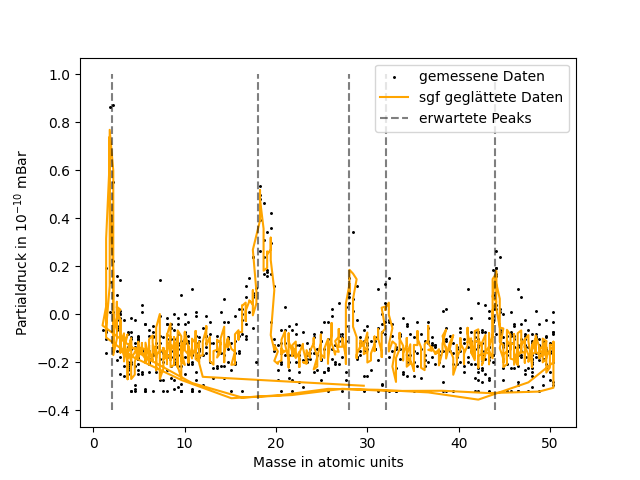
\includegraphics[width=140mm,scale=0.8]{Massenspektrometer/chapters/MSBreitspektrum.png}
    \caption{Spektrum der Raumluft im Massenbereich \SIrange[]{1}{51}{amu}}
    \label{fig:MSbreitspektrum}
\end{figure}

\begin{figure}
    \centering
    \includegraphics{}
    \caption{Caption}
    \label{fig:enter-label}
\end{figure}